\documentclass [t]{beamer}

\usepackage [T1]{fontenc}
\usepackage {ae,aecompl}
\usepackage [utf8]{inputenc}
\usepackage {graphicx}
\usepackage {url}
\usepackage {amsmath, amsfonts, amssymb}
\usepackage {booktabs}
\usepackage {tikz}
\usetikzlibrary{arrows,shapes,trees,shadows,positioning}

\usepackage {color}
\definecolor {rot}{RGB}{226,0,38}
\definecolor {blau}{RGB}{10,50,80}
\definecolor {gruen}{RGB}{157,193,7}
\definecolor {orange}{RGB}{243,154,38}
\definecolor {gelb}{RGB}{254,205,27}

\usetheme {Boadilla}
\usecolortheme {guix}
\usefonttheme [onlymath]{serif}

\setbeamertemplate {navigation symbols}{}
% zeige Gesamtseitenzahl nicht an; outhertheme-infolines entnommen und modifiziert
\setbeamertemplate{footline}
{
  \leavevmode%
  \hbox{%
  \begin{beamercolorbox}[wd=.333333\paperwidth,ht=2.25ex,dp=1ex,center]{author in head/foot}%
    \usebeamerfont{author in head/foot}\insertshortauthor~~(\insertshortinstitute)
  \end{beamercolorbox}%
  \begin{beamercolorbox}[wd=.333333\paperwidth,ht=2.25ex,dp=1ex,center]{title in head/foot}%
    \usebeamerfont{title in head/foot}\insertshorttitle
  \end{beamercolorbox}%
  \begin{beamercolorbox}[wd=.333333\paperwidth,ht=2.25ex,dp=1ex,right]{date in head/foot}%
    \usebeamerfont{date in head/foot}\insertshortdate{}\hspace*{2em}
    \insertframenumber{}\hspace*{2ex}
%    \insertframenumber{} / \inserttotalframenumber\hspace*{2ex}
  \end{beamercolorbox}}%
  \vskip0pt%
}

\AtBeginSection[]
{
  \begin{frame}
    \frametitle{\inserttitle}
    \tableofcontents[currentsection]
  \end{frame}
  \addtocounter {framenumber}{-1}
}


\begin{document}

\title [GNU Guix]{Packaging and deploying with GNU Guix and GuixSD}
\author {Andreas Enge}
\institute[INRIA Bordeaux]{LFANT project-team \\
INRIA Bordeaux--Sud-Ouest \\
\url {andreas.enge@inria.fr} \\
\url {http://www.math.u-bordeaux.fr/~aenge}}
\date [Sage Days 2016]{\color {gruen}Sage Days 77,
Cernay, 5 April 2016
}


\begin {frame}{}
\maketitle
\end {frame}


\setcounter {framenumber}{0}

\section* {Introduction}

\begin {frame}{Upgrades are difficult}
\includegraphics [width=11cm]{images/debian-upgrade-instructions.png}
\vfill
\tiny
\hfill \url {https://www.debian.org/releases/squeeze/amd64/release-notes/ch-upgrading.en.html}
\end {frame}


\begin {frame}{Upgrades are dangerous}
\includegraphics [width=11cm]{images/debian-upgrade-warning.png}
\vfill
\tiny
\hfill \url {https://wiki.debian.org/DebianPackageManagement}
\end {frame}


\begin{frame}[fragile]{Stateful system management is unpredictable}
  \begin{overlayarea}{\textwidth}{8cm}
  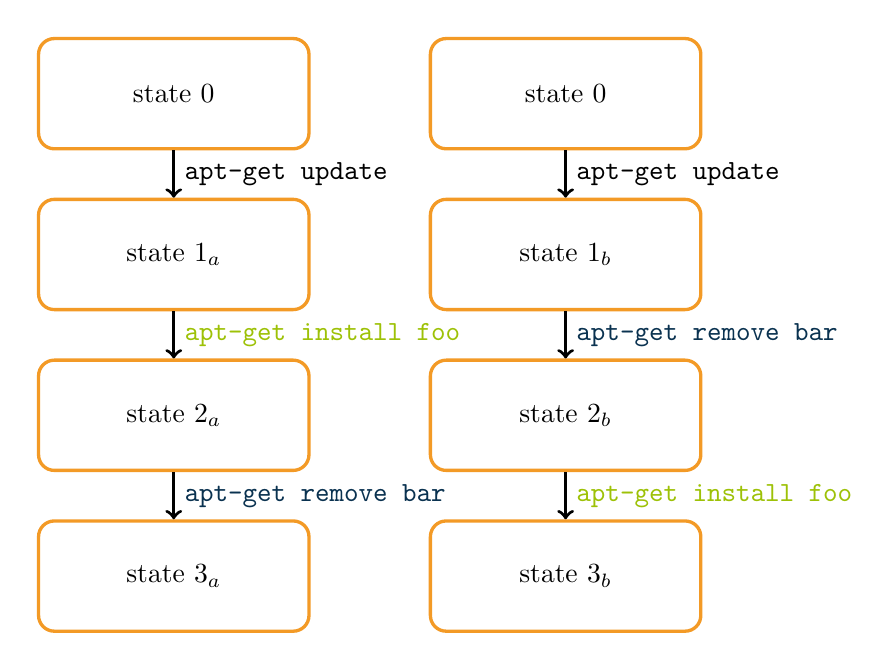
\begin{tikzpicture}[stylish/.style = {
                        draw=orange, very thick,
                        fill=white, text=black, text width=3.2cm,
                        rounded corners=2mm, minimum height=1.4cm,
                        text centered
                      }]
    \matrix[row sep=6mm, column sep=1.5cm] {
      \node(inita)[stylish]{state 0};
      & \node(initb)[stylish]{state 0};
      \\

      \node<2->(state1a)[stylish]{state $1_a$};
      & \node<2->(state1b)[stylish]{state $1_b$};
      \\

      \node<3->(state2a)[stylish]{state $2_a$};
      & \node<3->(state2b)[stylish]{state $2_b$};
      \\

      \node<3->(state3a)[stylish]{state $3_a$};
      & \node<3->(state3b)[stylish]{state $3_b$};
      \\
    };

    \path[->, very thick]<2->
      (inita) edge node[right]{\texttt{apt-get update}} (state1a);
    \path[->, very thick]<3->
      (state1a) edge node[right]{\textcolor {gruen}{\texttt{apt-get install foo}}} (state2a);
    \path[->, very thick]<3->
      (state2a) edge node[right]{\textcolor {blau}{\texttt{apt-get remove bar}}} (state3a);

    \path[->, very thick]<2->
      (initb) edge node[right]{\texttt{apt-get update}} (state1b);
    \path[->, very thick]<3->
      (state1b) edge node[right]{\textcolor {blau}{\texttt{apt-get remove bar}}} (state2b);
    \path[->, very thick]<3->
      (state2b) edge node[right]{\textcolor {gruen}{\texttt{apt-get install foo}}} (state3b);
  \end{tikzpicture}
  \end{overlayarea}

  \begin{tikzpicture}[overlay]
    \node<4>[rounded corners=4, text centered,
          fill=orange, text width=3cm,
          inner sep=5mm, opacity=.75, text opacity=1,
          drop shadow={opacity=0.5}] at (5, 4) {
            \textbf{\Huge{= ?}}
          };
  \end{tikzpicture}
\end{frame}


\begin {frame}{Too many cooks spoil the broth}
\includegraphics [width=11cm]{images/package-managers.png}
\vfill
\tiny
\hfill \url
{https://en.wikipedia.org/wiki/List_of_software_package_management_systems}
\end {frame}


\begin {frame}{Fashionable solution: Give up}
\includegraphics [width=10cm]{images/docker-security.png}
\end {frame}


\begin{frame}[plain]
  \begin{tikzpicture}[remember picture, overlay]
    \node [at=(current page.center), inner sep=0pt]
          {\includegraphics[height=\paperheight]{images/hope-hero}};
  \end{tikzpicture}
\end{frame}



\section {GNU Guix: Principles and package management}

\begin {frame}{Functional package management}
\begin {eqnarray*}
\text {pari-gp}  & = & f_1 (\text {pari-2.7.5.tar.gz}, \text {readline},
  \text {gcc-5}, \text {make}) \\
\pause
\text {readline} & = & f_2 (\text {readline-6.3.tar.gz}, \text {ncurses},
  \text {gcc-5}, \text {make}) \\
\text {ncurses} & = & f_3 (\text {ncurses-6.0.tar.gz},
  \text {gcc-5}, \text {make}) \\
\pause
\text {gcc-5} & = & f_4 (\text {gcc-5.3.0.tar.gz},
  \text {gcc-4.9}, \text {make})
\end {eqnarray*}

\pause
\vspace {1cm}
Full \textcolor {blau}{directed acyclic graph} of dependencies is captured, \\
with a few \textcolor {rot}{bootstrap binaries} at the root.
\end {frame}


\begin{frame}[fragile]{The store}
  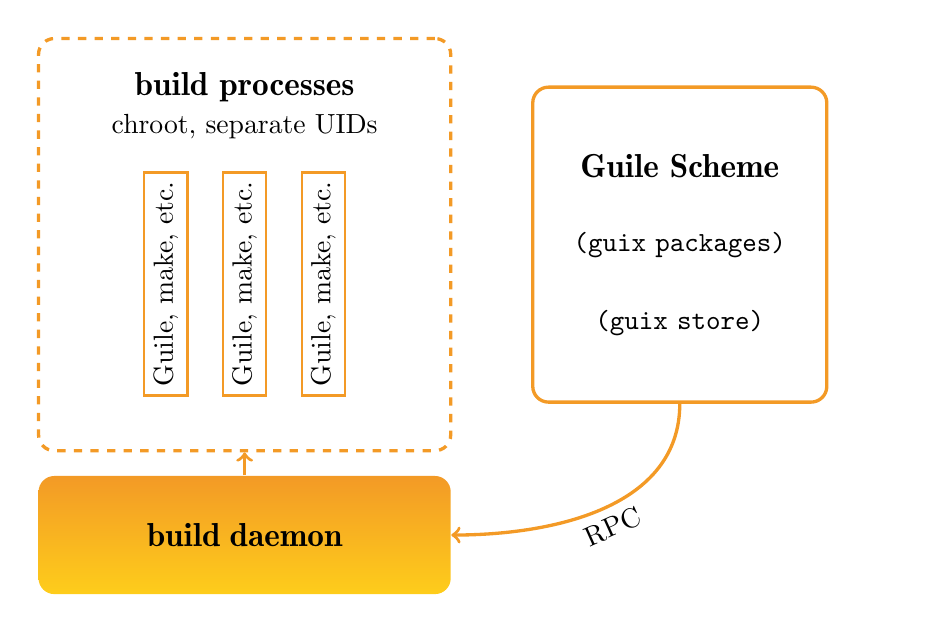
\begin{tikzpicture}[tools/.style = {
                        draw=orange, very thick,
                        text width=35mm, minimum height=4cm,
                        text centered,
                        rounded corners=2mm
                      },
                      tool/.style = {
                        text width=3cm,
                        text centered
                      },
                      daemon/.style = {
                        rectangle, text width=50mm, text centered,
                        rounded corners=2mm, minimum height=15mm,
                        top color=orange,
                        bottom color=gelb
                      },
                      builders/.style = {
                        draw=orange, very thick, dashed,
                        text width=5cm,
                        rounded corners=2mm,
                      },
                      builder/.style = {
                        draw=orange, thick, rectangle,
                        rotate=90
                      }]
    \matrix[row sep=3mm, column sep=1cm] {
      \node(builders)[builders, text height=5cm]{}
          node at (0, 2) {\large{\textbf{build processes}}}
          node at (0, 1.5) {chroot, separate UIDs}
          node[builder] at (-1,-0.5) {Guile, make, etc.}
          node[builder] at ( 0,-0.5) {Guile, make, etc.}
          node[builder] at ( 1,-0.5) {Guile, make, etc.}; &
      \node(tools)[tools]{}
          node at (0, 1) {\large{\textbf{Guile Scheme}}}
          node[tool] at (0, 0) {\texttt{(guix packages)}}
          node(client)[tool] at (0, -1) {\texttt{(guix store)}};
      \\

      \node(daemon)[daemon]{\large{\textbf{build daemon}}}; &
      &
      \\
    };

    \path[very thick, draw=orange]
      (tools.south) edge [out=-90, in=0, ->] node[below, sloped]{RPC} (daemon.east);
    \path[->, very thick, draw=orange]
      (daemon) edge (builders);
  \end{tikzpicture}
\end{frame}


\begin{frame}[fragile]{Package recipes}
\vspace {-5mm}
\scriptsize
\begin{verbatim}
(define-public pari-gp
  (package
   (name "pari-gp")
   (version "2.7.5")
   (source (origin
       (method url-fetch)
       (uri "http://pari.math.u-bordeaux.fr/pub/pari/unix/pari-2.7.5.tar.gz")
       (sha256 (base32 "0c8l83a0gjq73r9hndsrzkypwxvnnm4pxkkzbg6jm95m80nzwh11"))))
   (build-system gnu-build-system)
   (inputs `(("gmp" ,gmp)
             ("libx11" ,libx11)
             ("perl" ,perl)
             ("readline" ,readline)))
   (arguments
    '(#:make-flags '("gp")
      #:test-target "dobench"
      #:phases (modify-phases %standard-phases
       (replace 'configure
         (lambda* (#:key outputs #:allow-other-keys)
           (system* "./Configure"
                    (string-append "--prefix=" (assoc-ref outputs "out"))))))))
   (license license:gpl2+)
   (home-page "http://pari.math.u-bordeaux.fr/")))
\end{verbatim}
\end{frame}


\begin {frame}{\texttt {guix graph --type=packages pari-gp}}
\includegraphics [width=12cm]{images/graph-parigp-packages.pdf}

\vfill
And gcc, make and so on? Implicit inputs!
\end {frame}


\begin {frame}{\texttt {guix graph --type=bag-emerged pari-gp}}
\includegraphics [height=8cm,width=12cm]{images/graph-parigp-bag-emerged.pdf}
\end {frame}


\begin{frame}[fragile]{Demo: Packages and profiles}
\small
\begin {itemize}
\item
\texttt {guix build pari-gp}

\texttt {/gnu/store/\textcolor {orange}{qbb9f5s6xzbgac9f260g16b68j7w1wqb}-pari-gp-2.7.5}

Hash of all inputs!

\pause
\item
\texttt {guix gc -\,-references /gnu/store/-...-pari-gp-2.7.5}

\pause
\item
\texttt {guix package -i pari-gp}

Look at \texttt {\$HOME/.guix-profile}; run \texttt {gp}.

\pause
\item
\texttt {./pre-inst-env guix edit pari-gp}

\texttt {./pre-inst-env guix build pari-gp}

\texttt {guix gc -\,-references ...}

\texttt {./pre-inst-env guix package -u pari-gp}

\pause
\item
\texttt {guix package -l}

\pause
\item
\textcolor {gruen}{\texttt {guix package -\,-roll-back}}
\end {itemize}
\end{frame}


\begin {frame}{Features}
\begin {itemize}
\item
\textcolor {blau}{Hackable}
\begin {itemize}
\item
based on Guile Scheme
\end {itemize}
\item
\textcolor {blau}{Dependable}
\begin {itemize}
\item
immutable packages in store
\item
transactional upgrades \textcolor {gruen}{and downgrades}
\end {itemize}
\item
\textcolor {blau}{Liberating}
\begin {itemize}
\item
user centric: every user has an individual profile
\item
transparent (and reproducible?) binary and source deployments
\item
easy roll-back
\item
different versions can co-exist
\begin {itemize}
\item
in \textcolor {gruen}{one user profile} (?)
\item
for \textcolor {gruen}{different users}
\item
for one user in \textcolor {gruen}{different profiles}
\end {itemize}
\end {itemize}
\end {itemize}
\end {frame}



\section {GNU GuixSD: Declarative system deployments}

\begin {frame}{System layers}
\hspace {2cm}
  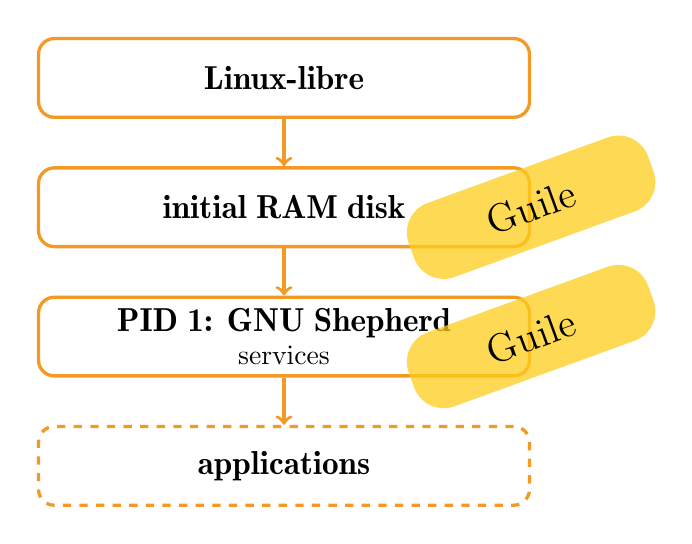
\begin{tikzpicture}[entry/.style = {
                        draw=orange, very thick,
                        fill=white, text=black, text width=6cm,
                        rounded corners=2mm, minimum height=1cm,
                        text centered
                      },
                      guile/.style = {
                         fill=gelb, text=black, rotate=20,
                         rounded corners=4mm, text width=3cm,
                         opacity=.75, text opacity=1, text centered,
                         minimum height=1cm
                      }]
    \matrix[row sep=6mm, column sep=1cm] {
      \node(kernel)[entry]{\textbf{\large{Linux-libre}}};
      \\
      \node(initrd)[entry]{\textbf{\large{initial RAM disk}}};
      \\

      \node(shepherd)[entry]{\textbf{\large{PID 1: GNU Shepherd}}
        \\ services};
      \\

      \node(user)[entry, dashed]{\textbf{\large{applications}}};
      \\
    };

    \path[->, very thick, draw=orange]
      (kernel) edge (initrd);
    \path[->, very thick, draw=orange]
      (initrd) edge (shepherd);
    \path[->, very thick, draw=orange]
      (shepherd) edge (user);

    \node<2->(labelinitrd) [guile] at (initrd.east) {%
      \Large{Guile}
    };
    \node<2->(labelinitrd) [guile] at (shepherd.east) {%
      \Large{Guile}
    };
  \end{tikzpicture}
\end {frame}


\begin {frame}{Demo: Always change a running system!}
Have a look at

\texttt {/run}

\texttt {/run/current-system}

\texttt {/run/booted-system}

\texttt {/run/current-system/}
\end {frame}


\begin {frame}{Demo: Do as you please!}
\begin {itemize}
\item
Look at \texttt {config-desktop.scm}.
\pause
\item
Change!
\begin {itemize}
\item
change locales
\item
add pari-gp package to global list
\item
auto-login the user \texttt {enge}
\end {itemize}

\pause
\item
\texttt {guix system vm config-pari.scm}

\pause
\item
\texttt {guix system reconfigure config-pari.scm}
\end {itemize}
\end {frame}


\section {State of the nation}

\begin {frame}{Timeline}
\begin {itemize}
\item
2012-11: GNU project by Ludovic Courtès
\item
2013-01: release 0.1
\item
2014-07: \textcolor {blau}{installable operating system}
\item
2015-01: ARMv7 port
\item
2016-01: successful fundraiser for new build farm
\item
2016-02: creation of \textcolor {blau}{Guix Europe}, \\
non-profit organisation to support GNU Guix
\item
2016-03: release 0.10.0
\end {itemize}
\end {frame}


\begin {frame}{Status and activities}
\begin {itemize}
\item
3200 packages
\item
4 platforms
\begin {itemize}
\item
GuixSD: x86\_64, i686
\item
Guix as package manager: mips64el, armhf
\end {itemize}
\item
$\approx$ 25 contributors per month
\item
$\approx$ 400 commits per month
\item
lots of friendly people on the mailing list and on IRC
\end {itemize}

\pause
\vfill
\begin {center}
\color {rot}\framebox {\textcolor {orange}{Try it out!}}
\end {center}
\begin {itemize}
\item
\url {https://gnu.org/software/guix/}
\item
It is free
\begin {itemize}
\item
as in \textcolor {gruen}{libre}
\item
of \textcolor {orange}{cost}
\item
of \textcolor {rot}{risk}
\end {itemize}
\end {itemize}
\end {frame}


\begin {frame}
\centerline {\includegraphics[width=0.3\textwidth,angle=270]{images/guixsd.pdf}}

\vfill
    \tiny{
      Copyright \copyright{} 2016 Andreas Enge \texttt{andreas.enge@inria.fr}\\
      Some slides are \copyright{} 2010, 2012--2016 Ludovic Courtès \texttt{ludo@gnu.org}\\[2mm]

      GNU GuixSD logo \copyright{} 2015 Luis Felipe López Acevedo <felipe.lopez@opmbx.org>\\
      CC-BY-SA 4.0, \url{http://gnu.org/s/guix/graphics}\\[2mm]

      Copyright of other images included in this document is held by
      their respective owners.
      \\[2mm]
      This work is licensed under the \alert{Creative Commons
        Attribution-Share Alike 3.0} License.  To view a copy of this
      license, visit
      \url{http://creativecommons.org/licenses/by-sa/3.0/} or send a
      letter to Creative Commons, 171 Second Street, Suite 300, San
      Francisco, California, 94105, USA.
      \\[2.0mm]
      At your option, you may instead copy, distribute and/or modify
      this document under the terms of the \alert{GNU Free Documentation
        License, Version 1.3 or any later version} published by the Free
      Software Foundation; with no Invariant Sections, no Front-Cover
      Texts, and no Back-Cover Texts.  A copy of the license is
      available at \url{http://www.gnu.org/licenses/gfdl.html}.
      \\[2.0mm]
      % Give a link to the 'Transparent Copy', as per Section 3 of the GFDL.
      The source of this document is available from
      \url{http://git.sv.gnu.org/cgit/guix/maintenance.git}.
    }
\end {frame}

\end {document}
